\chapter{Implementation}\label{ch:implementation}
% WORD BUDGET: ~1200 words (12k total target; COMP0234 limit UNVERIFIED — confirm on Moodle)

This chapter records the engineering that made the design measurable: the
simulated London networks, the on-device serving stack and its documented
failure modes, the distillation and compile chain, and the experiment
harness. I keep it tight and evidence-focused, with
Appendix~\ref{app:repro} tabulating the reproducibility pins (versions,
seeds, templates).


\subsection{Simulation environment and topologies}\label{sec:imp-sumo}
All control runs in SUMO with TraCI. Six topologies span a
regular-synthetic to irregular-real axis along which \S\ref{ch:results}
finds the largest differences, without isolating which property carries
them: two synthetic grids (3$\times$3, 4$\times$4), a Bloomsbury grid from
OpenStreetMap, the Euston A501 corridor and its peak-hour variant, and the
Old Street complex junction. Euston's AADF-derived demand carries the
A501's measured DfT vehicle mix but an assumed hourly profile, the
peak-hour variant rescaled to the measured DfT peak-hour magnitude. Old
Street's nine signals include a single five-arm, seventeen-movement
junction, demand-calibrated after default random demand gridlocked it, as
were the Bloomsbury grid and Euston peak-hour corridor
(\S\ref{sec:res-calib}). Only Euston's demand magnitude is measured, the
other two real maps being randomTrips draws (\S\ref{sec:dis-threats}).
Figure~\ref{fig:sumo-gui} shows the Bloomsbury network under the
calibrated demand.

\begin{figure}[t]
\centering
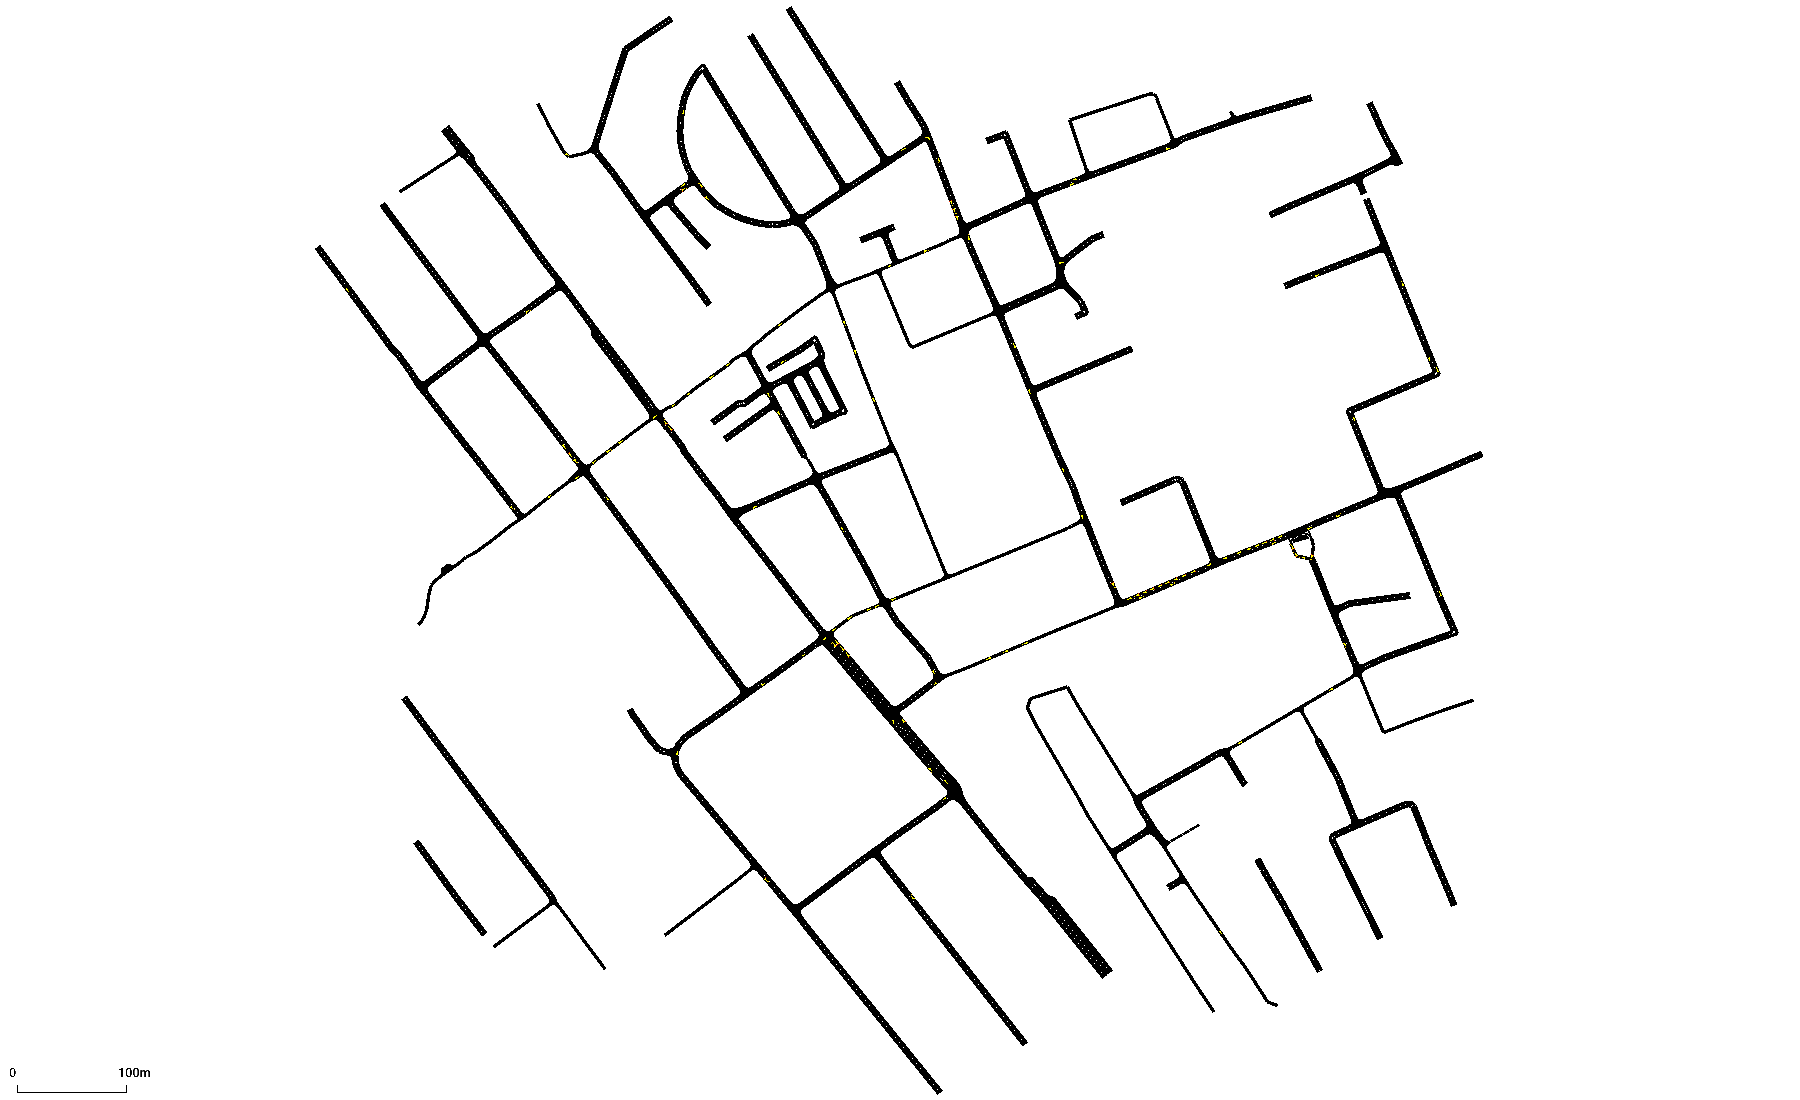
\includegraphics[width=\columnwidth]{figures/bloomsbury-sumo-gui.png}
\caption{The Bloomsbury network in SUMO at $t{=}420$\,s under the
calibrated 40\% demand (seed 1): nine signalised junctions extracted from
OpenStreetMap, 112 vehicles in motion.}
\label{fig:sumo-gui}
\end{figure}

\subsection{On-device serving with Foundry Local}\label{sec:imp-foundry}
Serving is Microsoft Foundry Local (pinned 0.8.119) on an RTX~2060 with
6\,GB VRAM, consumer hardware of roughly signal-cabinet class and a hard
project constraint: it caps the ladder at $\sim$4B (7B-class models OOM
the runtime, recorded), which makes the scale-saturation result
(\S\ref{sec:res-offline}) deployment-relevant rather than academic.

Custom models serve through two execution providers. The CPU path works
out of the box; WebGPU requires editing the compiled model's
\texttt{genai\_config.json} provider options and delivers about
$1.6\times$ lower latency at \emph{equal aggregate holdout accuracy} on the
one artifact and format where both providers were scored
(\S\ref{sec:res-offline}), which licensed running every sweep GPU-served.
That comparison is within one artifact, not a claim of absolute speed: my
pipeline-compiled 0.6B artifacts serve at roughly 2.6 times the median
latency of the vendor catalogue build of the same weights
(\S\ref{sec:res-reliability}), a real cost of controlling the compile
chain. Windows~ML CUDA autoregistration requires a newer Windows build than
this machine's, making WebGPU the effective GPU path. Three reliability
findings from sustained unattended serving are mitigated in harness
(\S\ref{sec:imp-harness}) and reported in \S\ref{sec:res-reliability}.

\subsection{Distillation dataset and training}\label{sec:imp-dataset}
From eight training-reserved seeds ($\{3, 7, 11, 29, 42, 57, 91, 123\}$) I
sampled 48{,}137 unique junction states across three separately sampled
pools: 16{,}988 delay-aware states that also render the privileged myopic
rows, 18{,}596 prediction and 12{,}553 coordination. A frontier teacher
labelled them, and a second frontier model re-labelled 600 of them in four
audit samples of 150, agreeing on 98.5\% (97.3--99.3\% per sample).
Rendering the four prompt formats over those pools yields 59{,}533
training examples and a hash-frozen holdout of 5{,}580
(\texttt{HOLDOUT\_MOD}=12), rendered family-aware (ChatML with an empty
think block and no-think marker for Qwen3, Qwen2.5's ChatML without the
marker, Phi's \texttt{<|system|>\ldots<|end|>} convention), with loss on
the completion only, targeting exactly \texttt{\{"phase": N\}}. Training
is QLoRA $r{=}16$, NF4 double quantisation, fp16 compute. The 0.6B student
trained on the serving machine itself (13.5\,h on the RTX~2060), so the
full loop from teacher to served controller fits on one consumer device;
the 3.8B student and its five ablation variants trained on a single UCL
RTX~4090 (2.3\,h each, 8.9M trainable parameters, 0.23\%).

\subsection{Compile-and-serve chain}\label{sec:imp-compile}
Six steps take merged bf16 weights to a served endpoint: QLoRA merge
$\to$ int4 RTN compile $\to$ config patch $\to$ manifest synthesis $\to$
cache registration $\to$ WebGPU provider swap. That chain is, to my
knowledge, the first documented end-to-end recipe for serving a custom
fine-tuned model through Foundry Local;
Appendix~\ref{app:repro} records each step with the failure that
established it.

\subsection{Experiment harness}\label{sec:imp-harness}
Two harnesses produced the closed-loop sweep and offline-evaluation
numbers: the \textbf{factorial runner} executes model $\times$ format
$\times$ topology $\times$ seed cells with per-cell raw JSON artifacts, a
pre-flight serving probe per cell and multi-pass retry for deferred cells,
and the \textbf{offline evaluator} scores holdout rows against the served
endpoint; standalone probes supplied the fixed-time floor, emergency
preemption, the attack battery, the crash-law audit, the authorisation
re-test and the retention probe. Both are fail-loud, resumable and
recoverable in the senses Appendix~\ref{app:repro} defines, and survived a
six-week unattended campaign including two service restarts, one machine
reboot and one mid-write power loss (one corrupted cell, detected by JSON
validation and re-run).

